\documentclass[a4paper,12pt]{article}
%

\usepackage{a4wide}
\usepackage{graphicx}
\usepackage{tikz}
\usetikzlibrary{shapes.geometric, arrows}
\usepackage[algo2e]{algorithm2e}
\usepackage{amsmath}
\usepackage{amsfonts}
\usepackage{amssymb}
\usepackage{multicol}
\usepackage{colortbl}
\usepackage{pgf,pgfarrows,pgfnodes,pgfautomata,pgfheaps,pgfshade}
\usepackage{gensymb}
\usepackage[utf8]{inputenc}
\usepackage[T1]{fontenc}
%\usepackage{dsfont}
\usetikzlibrary{shapes,trees}
\usetikzlibrary{graphs}
\usetikzlibrary{positioning}
\usetikzlibrary{arrows}
\usepackage{subcaption}
\usepackage[portuges]{babel}
\usepackage{siunitx}

\begin{document}
%
\title{Trabalho final de AGE e OSD}


\author{R. Vieira\thanks{Departamento de Engenharia Mecânica, Universidade do Minho, {\tt ae5333@alunos.uminho.pt}}}

\maketitle              % typeset the header of the contribution

\begin{abstract}
Este relatório destina-se a apresentar o trabalho das Unidades Curriculares (UCs) de Algoritmos Genéticos e Evolucionários (AGE) e Otimização Sem Derivadas (OSD). Inicia-se com a discrição do problema de otimização, originário da área de trabalho da minha bolsa de investigação. O prblema consiste em optimzar um sistema de teste para placas de circuito impresso quanto ao peso e rigidez. É apresentada uma discussão sobre a estrutura matemática do problema e a abordagem usada na sua resolução. Finaliza-se apresentando as conclusões.
\end{abstract}

\section{Introdução}

As placas de circuito impresso são essenciais numa era de crescente digitilização. É essencial garantir que não existem defeitos de produção para que operem normalmente na vida do componente. Para isso fazem-se testes com um sistema que mede tesnões e currentes no circuito. Devido ao facto de os circuitos serem da ordem dos \SI{70}{\micro\metre} é essencial que este sistema de teste tenha uma alta rigidez (pouca deformação em operação) e de baixo peso (para que os operadores troquem os sistemas de teste facilmente). 

Assim, as funções objetivo (a minimizar) são:


\begin{equation}\label{eq:deform}
w_0= \sum_{n=1}^{\infty} \sum_{m=1}^{\infty} W_{mn} sin\left(\frac{m \pi x}{a}\right) sin\left(\frac{n \pi y}{b}\right)
\end{equation}

\begin{equation}\label{eq:mass}
Mass = a b h \rho_{material}
\end{equation}

Ou seja, a massa do sistema equação~\ref{eq:mass} e os delocamentos que serão impostos pela carga na equação~\ref{eq:deform}. Sabendo que:

\begin{equation}\label{eq:fo}
D_{const}=\frac{E h^3}{12\left(1-{\nu}^2\right)}
\end{equation}

\begin{equation}\label{eq:fo}
k=\frac{k b^4}{D_{const} {\pi}^4}
\end{equation}

\begin{equation}\label{eq:fo}
\delta T=\frac{T \alpha D_{const} \left(1+\nu\right) {\pi}^2}{b^2}
\end{equation}

\begin{equation}\label{eq:fo}
W_{mn}=\frac{\frac{b^4}{D_{const} {\pi}^4} \left(q_{mn}+\delta T \left(m^2 s^2+n^2\right)\right)}{{\left(m^2 s^2+n^2\right)}^2+k}
\end{equation}

%\begin{equation}\label{eq:fo}
%\sigma_{max}=\frac{6q_mn\times2 b^2}{{\pi}^2 h^2 {\left(s^2+1\right)}^2} \left(s^2+\nu\right)
%\end{equation}

Para além disso, existem restrições tecnicas sobre os três parametros geométricos. O problema pode ser formalizado como:

\begin{equation}\label{eq:prob}
\begin{split}
\min\;\; &w_{0}(a, b, h)\\
\min\;\; &Mass(a, b, h)\\
s.a\;\; & 0.25\leq a\leq 0.5\\
& 0.25\leq b\leq 0.5\\
& 0.001\leq h\leq 0.01\\
\end{split}
\end{equation}

Onde $a$ e $b$ são os lados da chapa e $h$ é a sua espessura. Na figura~\ref{fig:defIm1}, vemos que a função deformação $w_{0}$ minimiza com a diminuição de $a$, $b$ e aumento de $h$.Nessa mesma figura é visivel que a função massa minimiza com os parametros $a$, $b$ e $h$. Ou seja, o parametro $h$ dá às funções um comportamento antagónico.Assim, o objectivo será conseguir um compromisso entre estas funções.

\begin{figure}[h]
\begin{center}
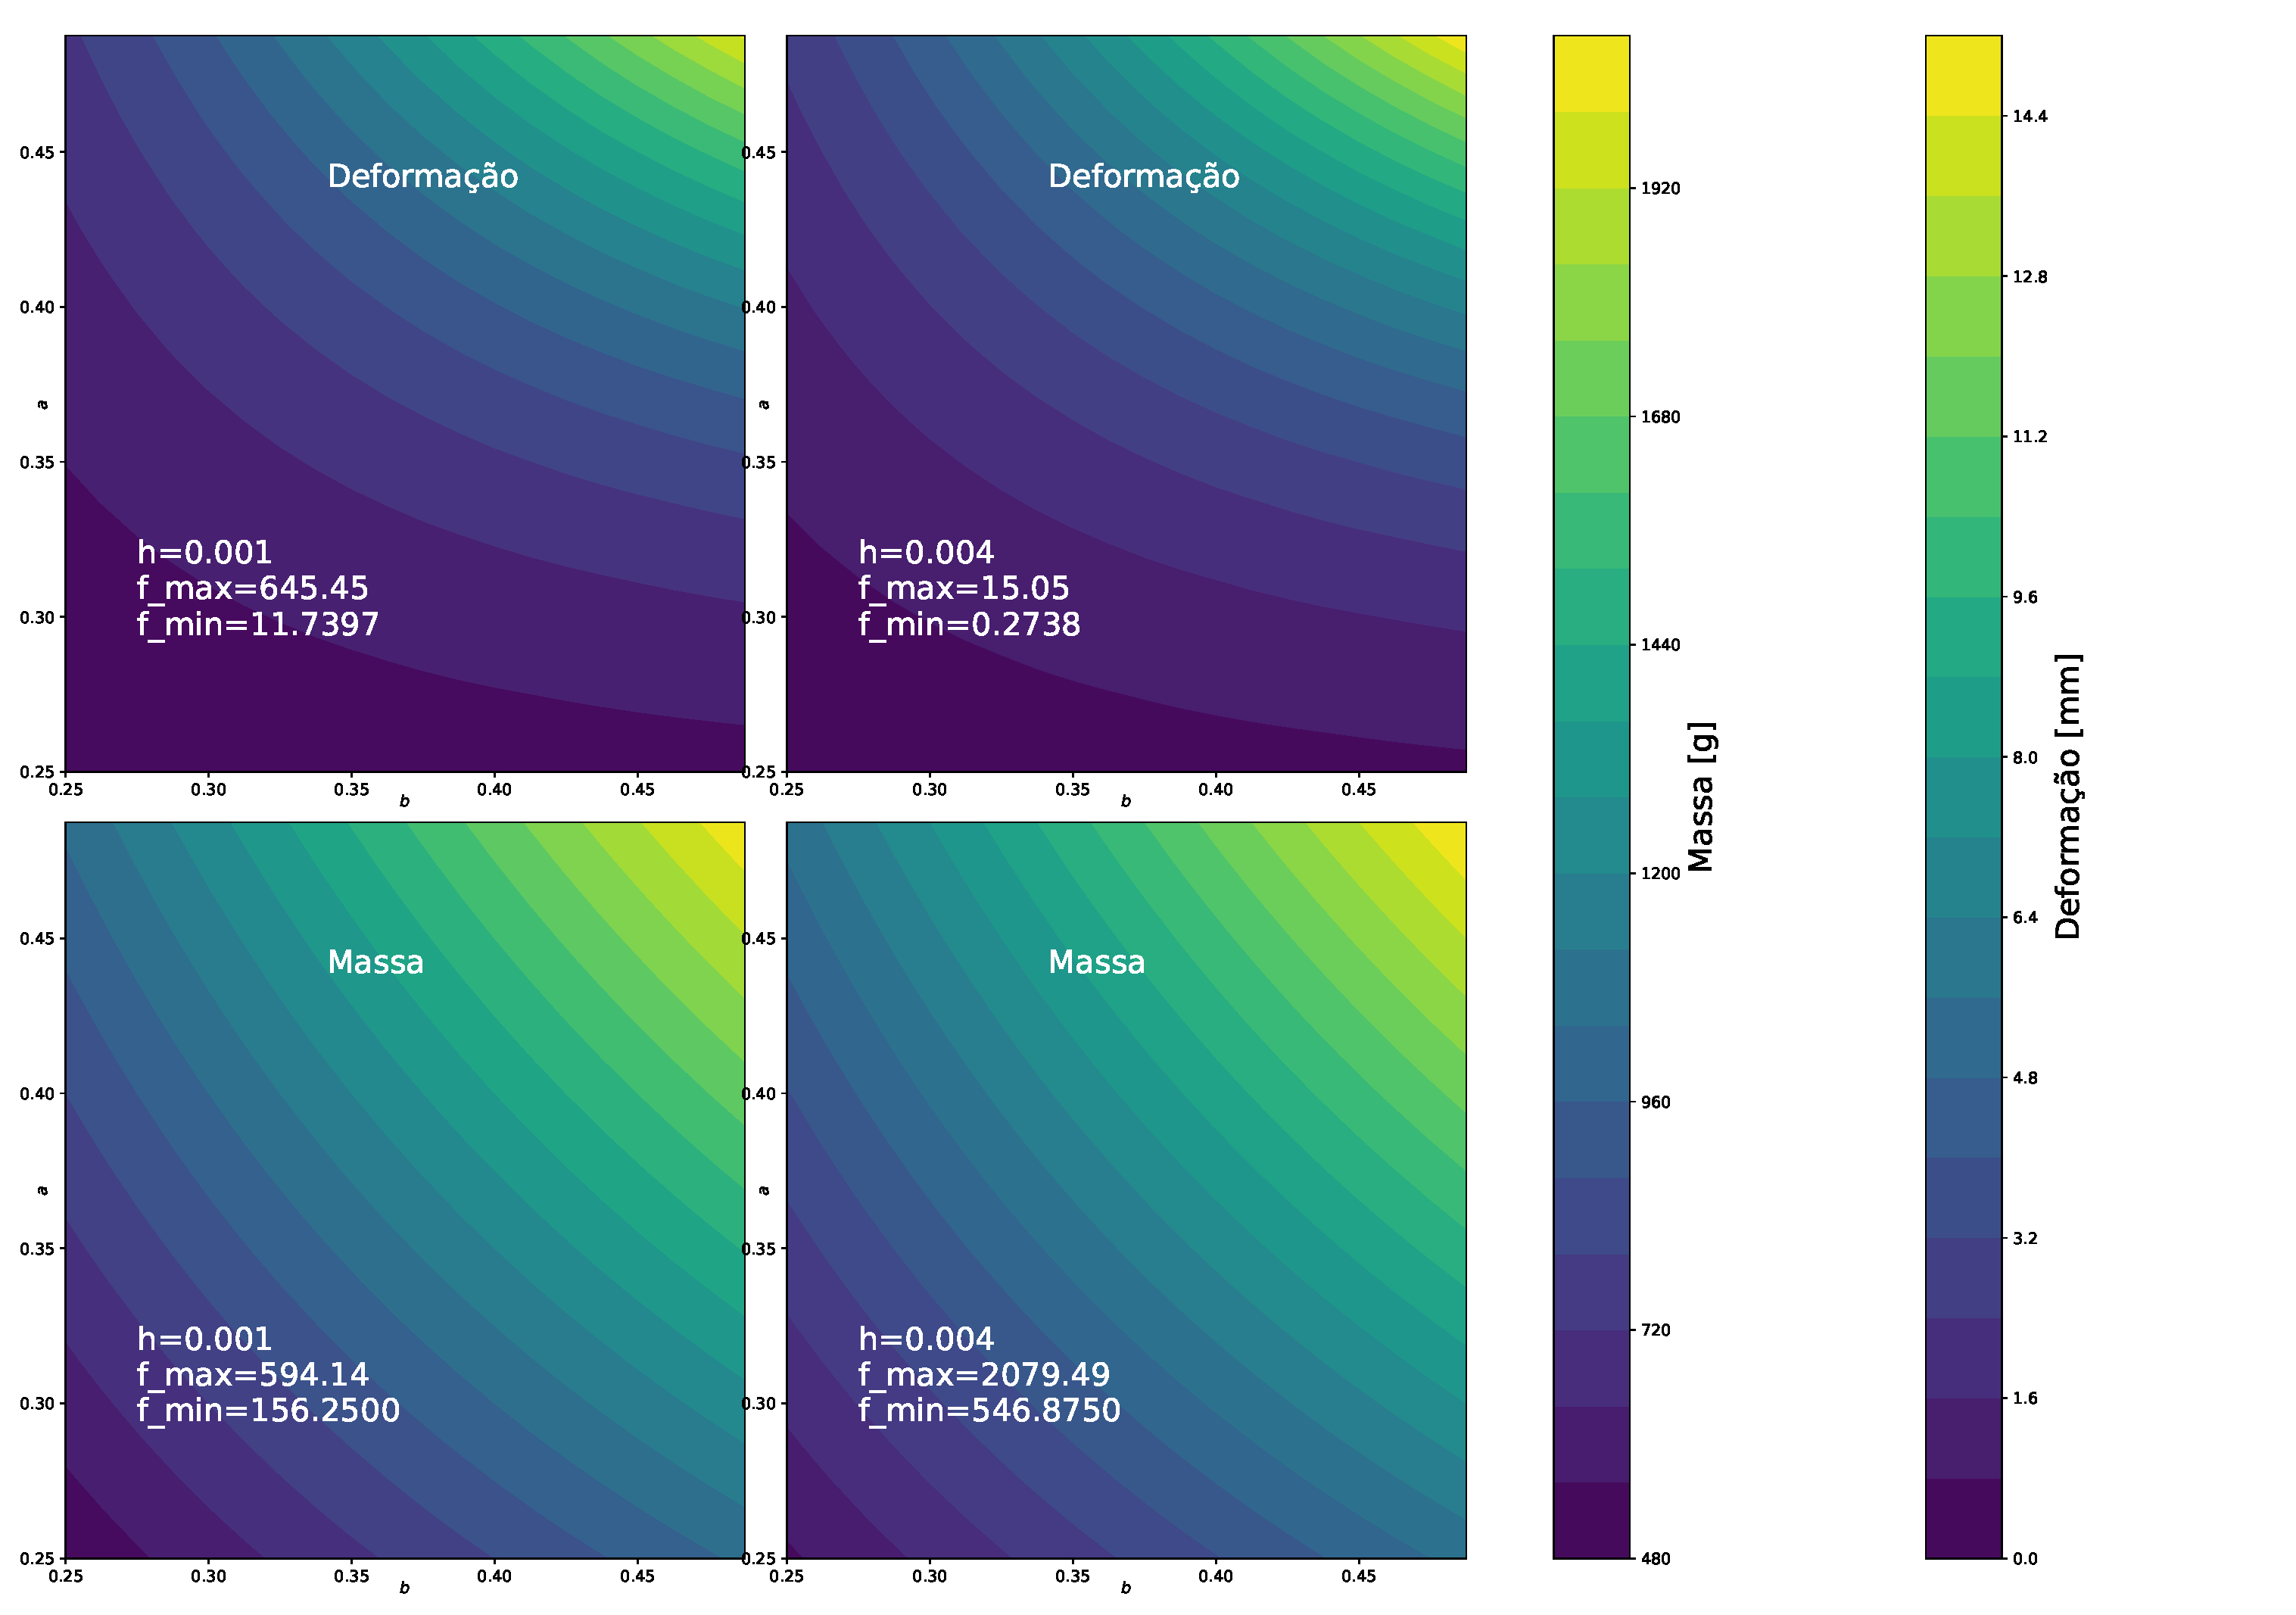
\includegraphics[scale=0.2]{deformacaoEmassa.eps}
\end{center}
\caption{A função massa e deformação desenhada com $h= 0.001, 0.004$}
\label{fig:defIm1}
\end{figure}

\section{Tecnica mais adequada para resolver o problema}




%Usar isto para a paralelos.
%
%\begin{figure}[!htbp]
%\centering
%\begin{subfigure}{.5\textwidth}
%  \centering
%  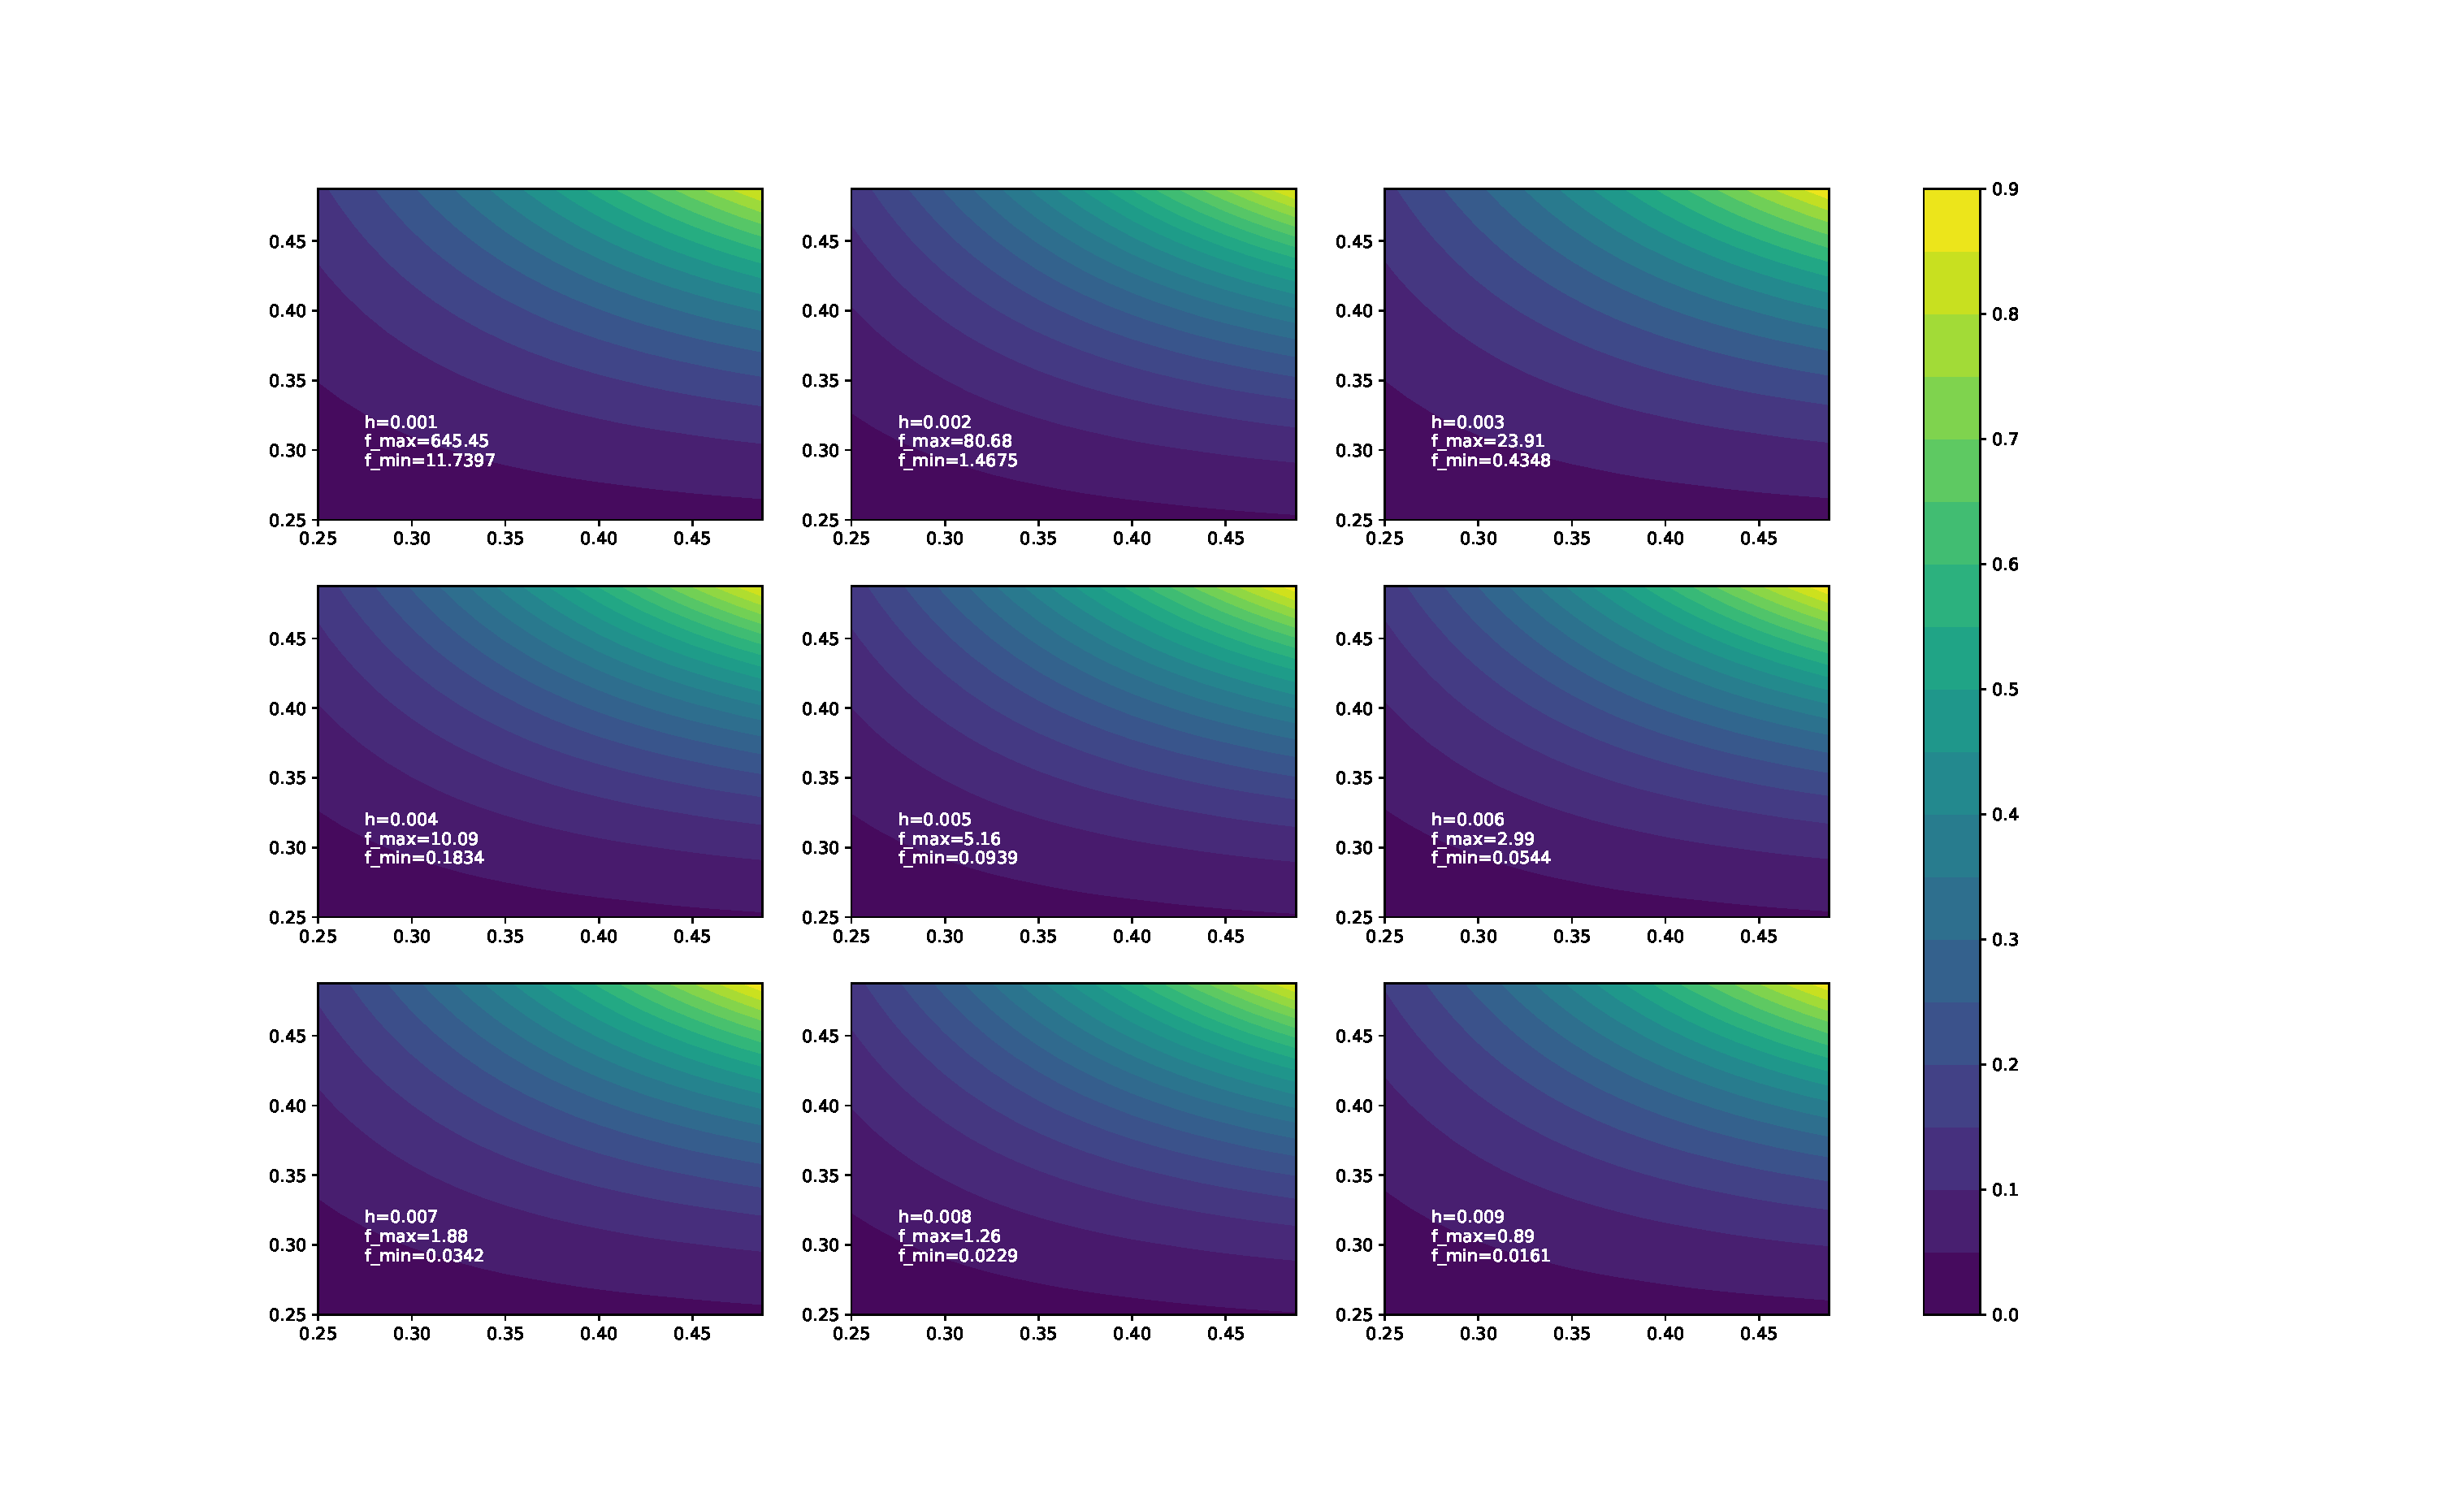
\includegraphics[width=.99\linewidth]{deformacao.eps}
%  \caption{Deformação}
%  \label{fig:sub1}
%\end{subfigure}%
%\begin{subfigure}{.5\textwidth}
%  \centering
%  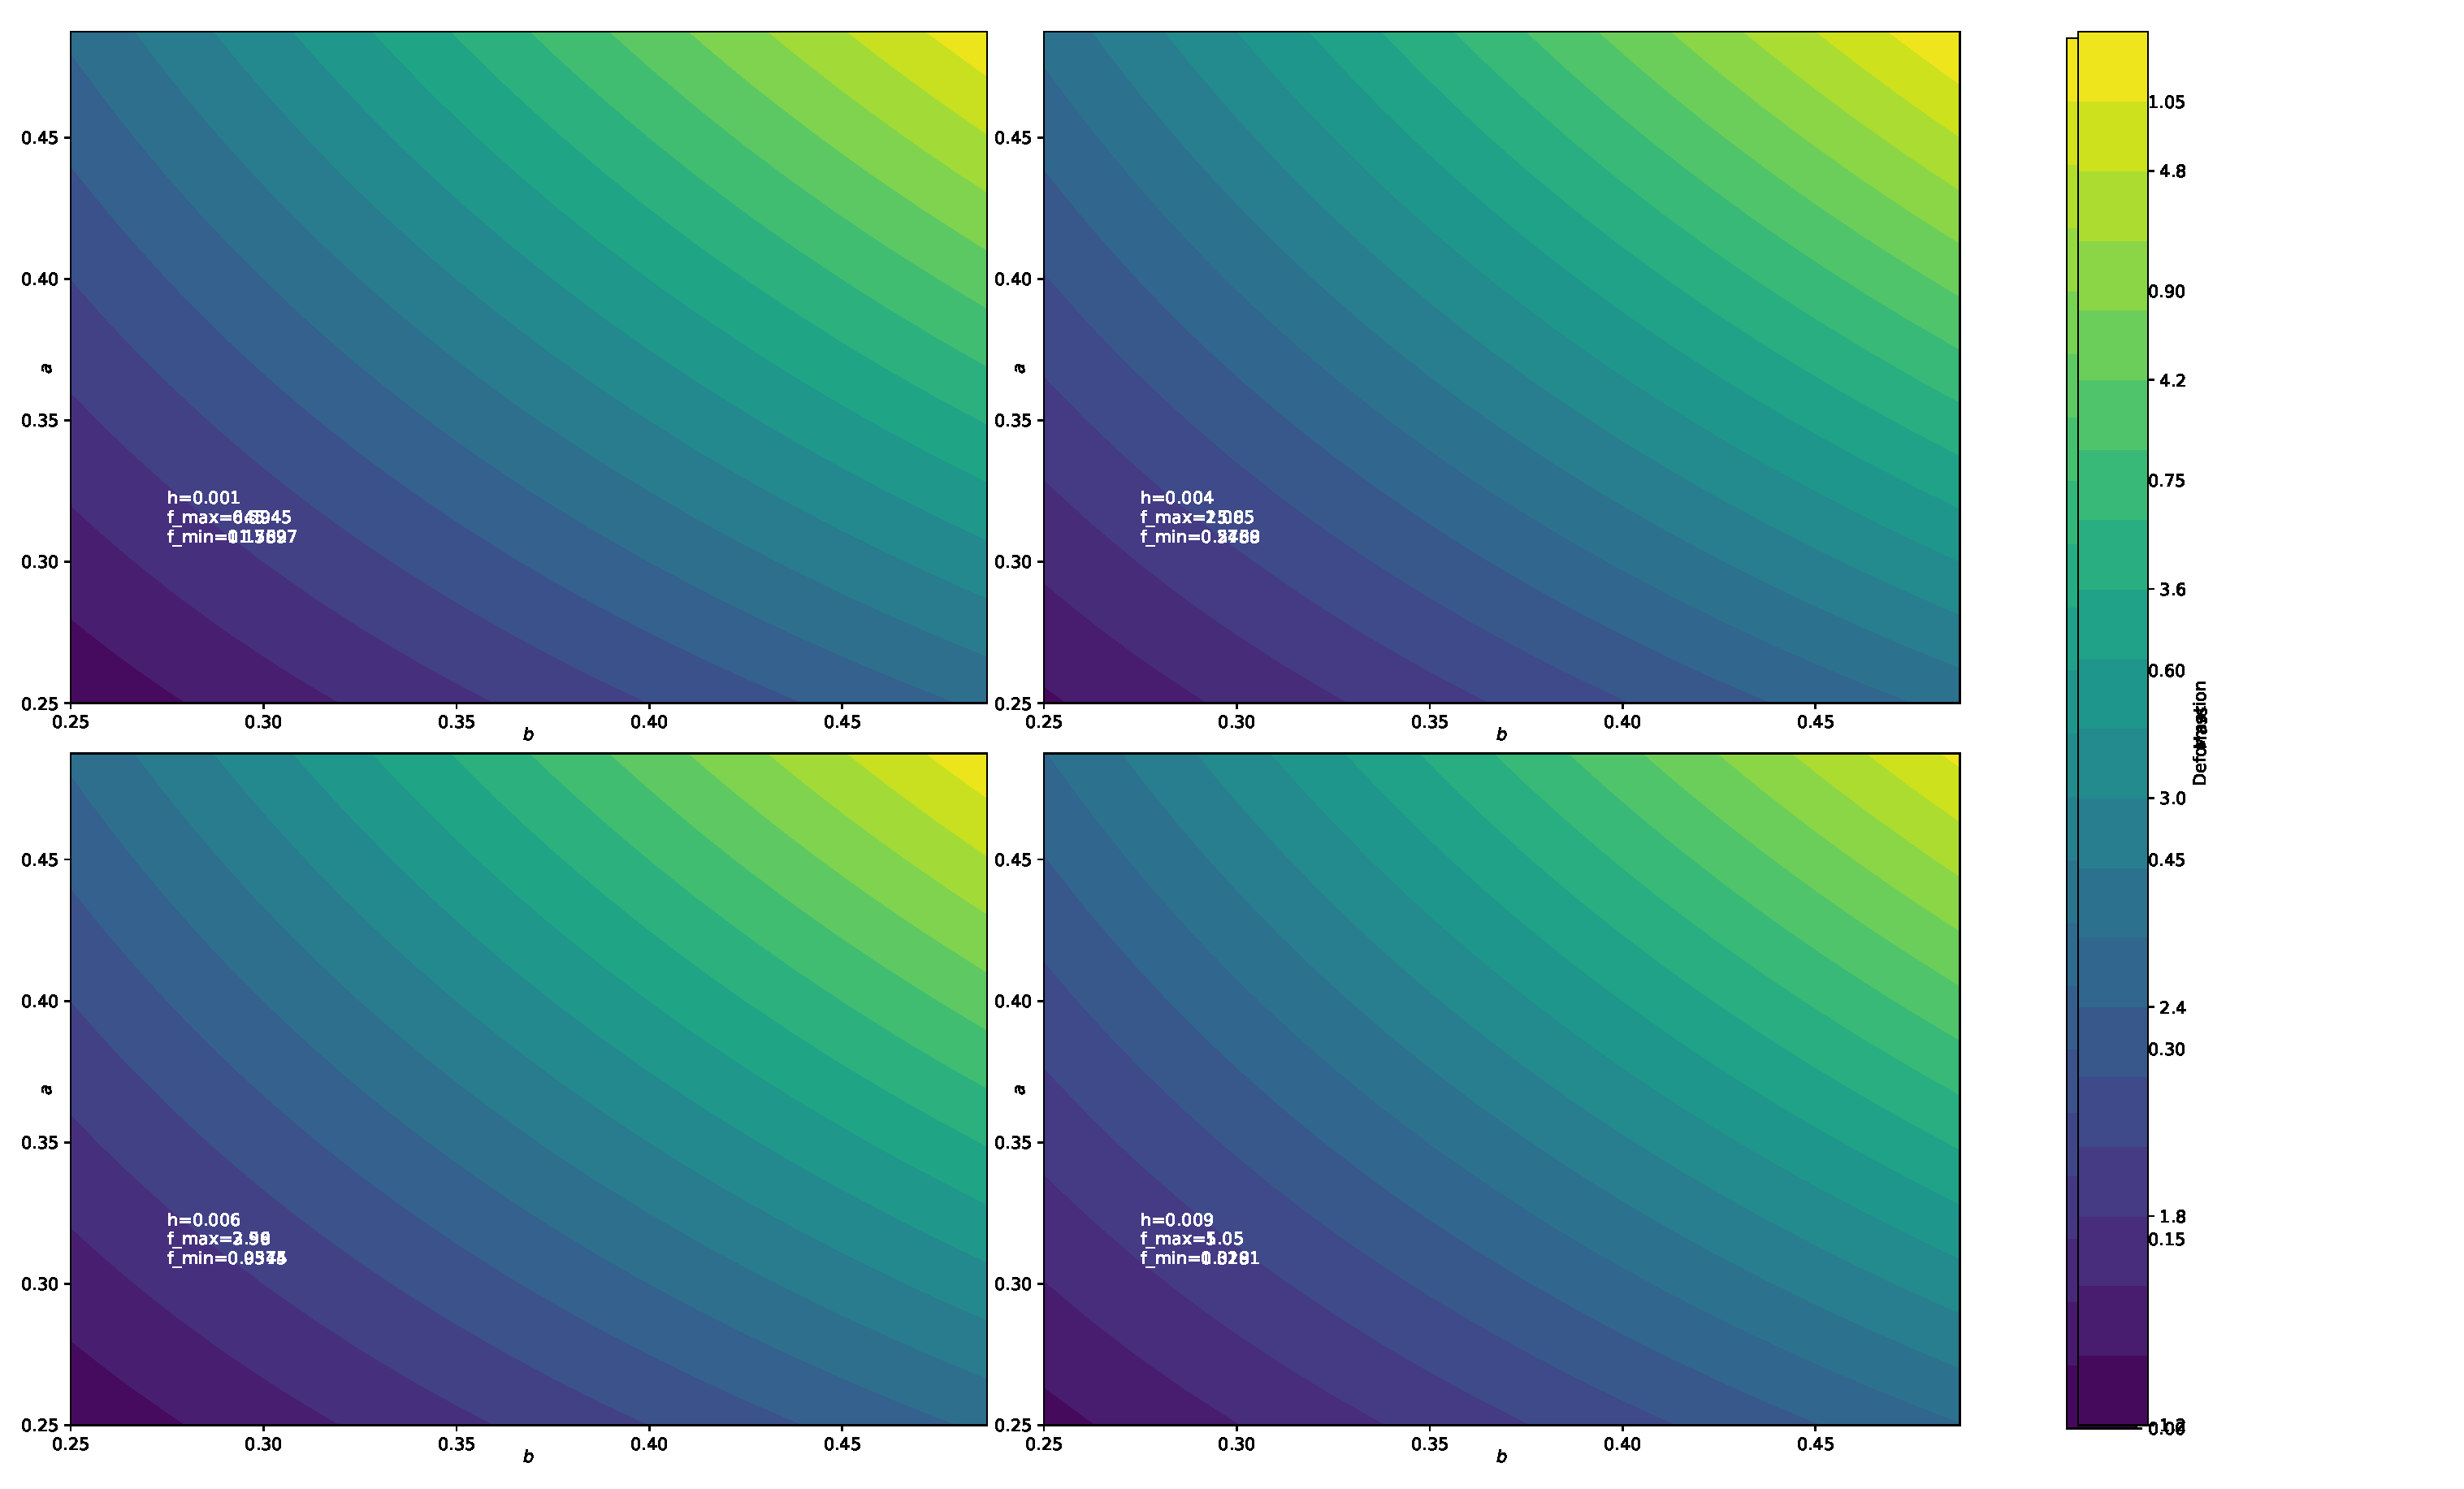
\includegraphics[width=.99\linewidth]{massa.eps}
%  \caption{Massa}
%  \label{fig:sub2}
%\end{subfigure}
%\caption{\label{fig:defIm2}A função desenhada com $z$ fixo ($z=2$)}
%%\label{fig:test}
%\end{figure}

\end{document}